%%%%%%%%%%%%%%%%%%%%%%%%%%%%%%%%%%%%%%%%%
% a0poster Portrait Poster
% LaTeX Template
% Version 1.0 (22/06/13)
%
% The a0poster class was created by:
% Gerlinde Kettl and Matthias Weiser (tex@kettl.de)
% 
% This template has been downloaded from:
% http://www.LaTeXTemplates.com
%
% License:
% CC BY-NC-SA 3.0 (http://creativecommons.org/licenses/by-nc-sa/3.0/)
%
%%%%%%%%%%%%%%%%%%%%%%%%%%%%%%%%%%%%%%%%%

%----------------------------------------------------------------------------------------
%	PACKAGES AND OTHER DOCUMENT CONFIGURATIONS
%----------------------------------------------------------------------------------------

\documentclass[a0,portrait]{a0poster}

\usepackage{multicol} % This is so we can have multiple columns of text side-by-side
\columnsep=100pt % This is the amount of white space between the columns in the poster
\columnseprule=3pt % This is the thickness of the black line between the columns in the poster

\usepackage[svgnames]{xcolor} % Specify colors by their 'svgnames', for a full list of all colors available see here: http://www.latextemplates.com/svgnames-colors

\usepackage{times} % Use the times font
%\usepackage{palatino} % Uncomment to use the Palatino font
\usepackage{subfig}
\usepackage{graphicx} % Required for including images
\graphicspath{{figures/}} % Location of the graphics files
\usepackage{booktabs} % Top and bottom rules for table
\usepackage[font=small,labelfont=bf]{caption} % Required for specifying captions to tables and figures
\usepackage{amsfonts, amsmath, amsthm, amssymb,eufrak} % For math fonts, symbols and environments
\usepackage{wrapfig} % Allows wrapping text around tables and figures
\usepackage{polski}
\usepackage[polish]{babel}
\usepackage[utf8]{inputenc}
\newtheorem{tw}{Twierdzenie}
\newtheorem*{theorem}{Twierdzenie}
\newtheorem{df}{Definicja}
\newtheorem*{defintion}{Definicja}
\newtheorem{lm}{Lemat}
\newtheorem*{lem}{Lemat}
\newtheorem{wn}{Wniosek}
\newtheorem{prz}{Przykład}
\newtheorem{uw}{Uwaga}
\newtheorem{za}{Założenie}
\newcommand{\norm}[1]{\left\lVert#1\right\rVert}
\DeclareFontShape{OMX}{cmex}{m}{n}{
  <-7.5> cmex7
  <7.5-8.5> cmex8
  <8.5-9.5> cmex9
  <9.5-> cmex10
}{}

\SetSymbolFont{largesymbols}{normal}{OMX}{cmex}{m}{n}
\SetSymbolFont{largesymbols}{bold}  {OMX}{cmex}{m}{n}

\begin{document}

%----------------------------------------------------------------------------------------
%	POSTER HEADER 
%----------------------------------------------------------------------------------------

% The header is divided into two boxes:
% The first is 75% wide and houses the title, subtitle, names, university/organization and contact information
% The second is 25% wide and houses a logo for your university/organization or a photo of you
% The widths of these boxes can be easily edited to accommodate your content as you see fit

\begin{minipage}[b]{0.75\linewidth}
\veryHuge \color{NavyBlue} \textbf{Dekonwolucja zaburzonego sygnału} \color{Black}\\ % Title
\Huge\textit{Podejście przez wyrocznie}\\[2cm] % Subtitle
\huge \textbf{Grzegorz Mika}\\[0.5cm] % Author(s)
\huge Akademia Górniczo-Hutnicza im. Stanisława Staszica w Krakowie\\[0.4cm] % University/organization
\Large \texttt{g.w.mika@gmail.com}\\
\end{minipage}
%
\begin{minipage}[b]{0.25\linewidth}

\includegraphics[width=9cm]{agh}\\
\end{minipage}

\vspace{1cm} % A bit of extra whitespace between the header and poster content

%----------------------------------------------------------------------------------------

\begin{multicols}{2} % This is how many columns your poster will be broken into, a portrait poster is generally split into 2 columns

%----------------------------------------------------------------------------------------
%	ABSTRACT
%----------------------------------------------------------------------------------------

\color{Navy} 

\begin{abstract}

Rozważony zostanie  problem estymacji nieznanego elementu $f$ na podstawie niebezpośrednich i zaburzonych obserwacji. Zaburzenie modelowane będzie przez pewien zwarty operator liniowy $A$. Niech $\Lambda$ będzie pewnym skończonym zbiorem estymatorów liniowych. Celem będzie konstrukcja metody wyboru estymatora z rodziny $\Lambda$ naśladującego estymator o minimalnym ryzyku w tej klasie. Okaże się, że można to osiągnąć poprzez minimalizację nieobciążonego estymatora ryzyka. W drugiej części zaprezentowany zostanie numeryczny przykład porównujący tę metodą z popularną metodą rozbieżności.
\end{abstract}

%----------------------------------------------------------------------------------------
%	INTRODUCTION
%----------------------------------------------------------------------------------------

\color{SaddleBrown} 

\section*{Wstęp}

Przypuśćmy, że obserwujemy zjawisko, w którym interesuje nas uzyskanie informacji na temat elementu $f$ należącego do pewnej przestrzeni Hilberta $\mathcal{H}$. Jednak w przeciwieństwie do klasycznych modeli nie obserwujemy sygnału $f$ bezpośrednio z pewnym błędem, a mamy dostęp jedynie do \textit{przekształconej} wersji z pewną niedokładnością. Zjawisko takie będzie modelowane w następujący sposób
\begin{displaymath}
Y=Af+\epsilon \xi,
\end{displaymath}
gdzie $Y$ jest obserwowane, $A$ jest zwartym operatorem liniowym  na $\mathcal{H}$, $\epsilon>0$ reprezentuje poziom szumu, natomiast $\xi$ jest gaussowskim białym szumem.\\
W rozważanym modelu, korzystając z reprezentacji singularnej SVD operatora $A$, możliwe jest zapisanie powyższego problemu w następującej postaci
\begin{displaymath}
y_n=b_n\theta_n+\epsilon\xi_n,\ n=1,2,\dots ,
\end{displaymath}
lub równoważnie
\begin{displaymath}
x_n=\theta_n+\epsilon\sigma_n\xi_n,\ n=1,2,\dots,
\end{displaymath}
gdzie $\xi_n\sim \mathcal{N}(0,1)$ są niezależnymi zmiennymi, $\theta_n$ są współczynnikami Fouriera funkcji $f$ w pewnej bazie ortonormalnej związanej z operatorem $A$, $x_n=y_n/b_n$, przy czym $b_n$ są wartościami singularnymi operatora $A$, natomiast ciąg $\sigma_n=1/b_n \to \infty$ związany jest ze złym uwarunkowaniem zadania, które pojawia się za każdym razem, gdy operator $A$ jest zwarty.\\
W ten sposób sprowadziliśmy zagadnienie do podobnego jak w przypadku regresji nieparametrycznej, czyli znalezienia dobrego estymatora dla współczynników $\theta_n$, jednak tym razem z uwagi na czynniki $\sigma_n$ sygnał ''ginie'' z czasem pośród szumu, który zaczyna dominować.


\color{Black} 

\section*{Teoria}
Calem odzyskania informacji o sygnale $f$ będziemy posługiwać się estymatorami liniowymi dla jego współczynników $\theta_n$.\\
Niech $\lambda=(\lambda_1,\lambda_2,\dots)$ będzie nielosowym ciągiem liczbowym. Estymatorem liniowym współczynników $\theta_n$ nazwiemy estymator $\hat{\theta(\lambda)}=(\hat{\theta_1},\hat{\theta_2},\dots)$, gdzie
\begin{displaymath}
\hat{\theta_i}=\lambda_ix_i,\ i=1,2,\dots.
\end{displaymath}
Ciąg $\lambda$ nazywać będziemy filtrem lub wagami.

Jakość estymatora $\hat{f}$ elementu $f$ mierzona będzie przy pomocy scałkowanego ryzyka średniokwadratowego
\begin{displaymath}
\mathcal{R}(\hat{f},f)=\mathbb{E}_f||f-\hat{f}||^2.
\end{displaymath}
W przypadku naszego modelu dostajemy, że 
\begin{displaymath}
\mathcal{R}(\hat{f},f)=\mathbb{E}_f||f-\hat{f}||^2=\mathbb{E}_{\theta} \Huge{\sum}_n \left(\theta_n-\hat{\theta}_n\right)^2=\mathbb{E}_{\theta}||\theta-\hat{\theta}||^2
\end{displaymath}
Gdy mamy do czynienia z estymatorem liniowym wyrażenie to sprowadza się do postaci 
\begin{displaymath}
\mathbb{E}_{\theta}||\theta-\hat{\theta}||^2
=\sum_{n=1}^{\infty}(1-\lambda_n)^2\theta_n^2+\epsilon^2\sum_{n=1}^{\infty}\sigma_n^2\lambda_n^2.
\end{displaymath}
Rozważać będziemy teraz pewien skończony zbiór estymatorów liniowych $\Lambda$.\\
Zaproponowane podejście opiera się na znalezieniu takiego filtra, by minimalizował on powyższe ryzyko. Jednak element taki wymagałby znajomości estymowanego elementu, zatem nie jest on dostępny dla statystyka. Element taki nazywany jest wyrocznią. Zamiast minimalizować zatem bezpośrednio ryzyko będziemy minimalizować jego nieobciążony estymator, a dokładniej nieobciążony estymator wyrażeni $\mathcal{R}(\hat{\theta},\theta)-\sum_{n=1}^{\infty}\theta_n^2$ postaci
\begin{displaymath}
U(\lambda,Y)=\sum_{n=1}^{\infty}(\lambda_n^2-2\lambda_n)x_n^2+2\epsilon^2\sum_{n=1}^{\infty}\lambda_n\sigma_n^2.
\end{displaymath}
Oznaczając przez $\lambda^*$ element minimalizujący $U(\lambda,Y)$ w zbiorze $\Lambda$ i wprowadzając oznaczenia \\
$\rho(\lambda)=\sup_n\sigma_n^2|\lambda_n|\left[\sum_{k=1}^{\infty}\sigma_k^4\lambda_k^4\right]^{-1/2}$, $\rho=\max_{\lambda\in \Lambda}\rho(\lambda)$, $S=\frac{\max_{\lambda\in\Lambda}\sup_n\sigma_n^2\lambda_n^2}{\min_{\lambda\in \Lambda}\sup_n\sigma_n^2\lambda_n^2}$, $M=\sum_{\lambda\in \Lambda}\exp\left(\frac{-1}{\rho(\lambda)}\right)$, $L_{\lambda}=\ln(NS)+\rho^2\ln^2(MS)$,
gdzie $N$ jest licznością zbioru $\Lambda$, otrzymujemy uzasadnienie zaproponowanej metody w postaci następującej nierówności wyroczni dla estymatora $\theta^*=\lambda^*Y$ przy odpowiednich założeniach
\begin{displaymath}
\mathbb{E}\norm{\theta^*-\theta}^2\leq (1+\gamma_1B^{-1})\min_{\lambda\in \Lambda}\mathcal{R}(\hat{\theta},\theta)+\gamma_2B\epsilon^2L_{\Lambda}\omega(B^2L_{\Lambda}),
\end{displaymath}
gdzie stałe $B>B_01>0,\gamma_1>0,\gamma_2>0$ niezależną od elementu $f$ i rodziny $\Lambda$, a funkcja $\omega(x)$ jest postaci
\begin{displaymath}
\omega(x)=\max_{\lambda\in \Lambda}\sup_k\left[\sigma_k^2\lambda_k^2\pmb{1}\left(\sum_{n=1}^{\infty}\sigma_n^2\lambda_n^2\leq x \sup_k\sigma_k^2\lambda_k^2\right)\right],\ x>0.
\end{displaymath}
Ryzyko zaproponowanego estymatora pozwala się zatem porównać z ryzykiem wyroczni.\\
Co ważne nierówność ta jest nieasymptotyczna, dając kryterium wyboru estymatora dla dowolnej wielkości próby.
\section*{Praktyka}
Rozważmy problem dekonwolucji funkcji $f$ na odcinku $[0,1]$ z zaburzonych obserwacji funkcji postaci
\begin{displaymath}
(Af)(s)=\int_0^1\phi (s-t)f(t)dt,
\end{displaymath}
gdzie jądro $\phi$ jest zdefiniowane następująco
\begin{displaymath}
\phi(t)=\frac{1}{\sqrt{2\pi a^2}}e^{-\frac{x^2}{2a^2}},\ a\in \mathbb{R}.
\end{displaymath} 
Za testową funkcję przyjęto funkcję postaci $f(t)=\left\{{-t,\ t<1/3}\atop {2x-1,\ x>1/3}\right.$, natomiast wartość parametru $a$ wybrano na poziomie $0.1$. 
\begin{center}

\includegraphics[width=0.4\linewidth]{f}
\captionof{figure}{\color{Green}Funkcja $f$ przed i po zniekształceniu}
\end{center}
Błąd $\epsilon\xi_n$ był generowany jako realizacja niezależnych zmiennych losowych o rozkładzie normalnym ze średnią zero i odchyleniem standardowym w wysokości $5\%$ maksymalnej wartości $Af$.\\
Rozważać będziemy teraz skończoną rodzinę estymatorów rzutowych z wagami postaci $\lambda_n=\pmb{1}\{n\leq N\}$, dla których jakości kluczowy jest wybór poziomu obcięcia $N$.\\
Metodą, do której porównana zostanie zaproponowana, jest zasada rozbieżności Morozowa. Gdybyśmy znali prawdziwy poziom błędu $\norm{y-y_0}=\epsilon$ optymalnym poziomem obcięcia byłby wtedy taki poziom $k$, że jest on najmniejszą taką liczbą, że zachodzi $||y-Af_k||<\epsilon$, gdzie $f_k$ jest rozwiązaniem uzyskanym z $\lambda_k$. Możemy zatem próbować estymować poziom szumu i na tej podstawie wybierać poziom obcięcia. Zastosowanie tej metody daje następujący rezultat
\begin{center}
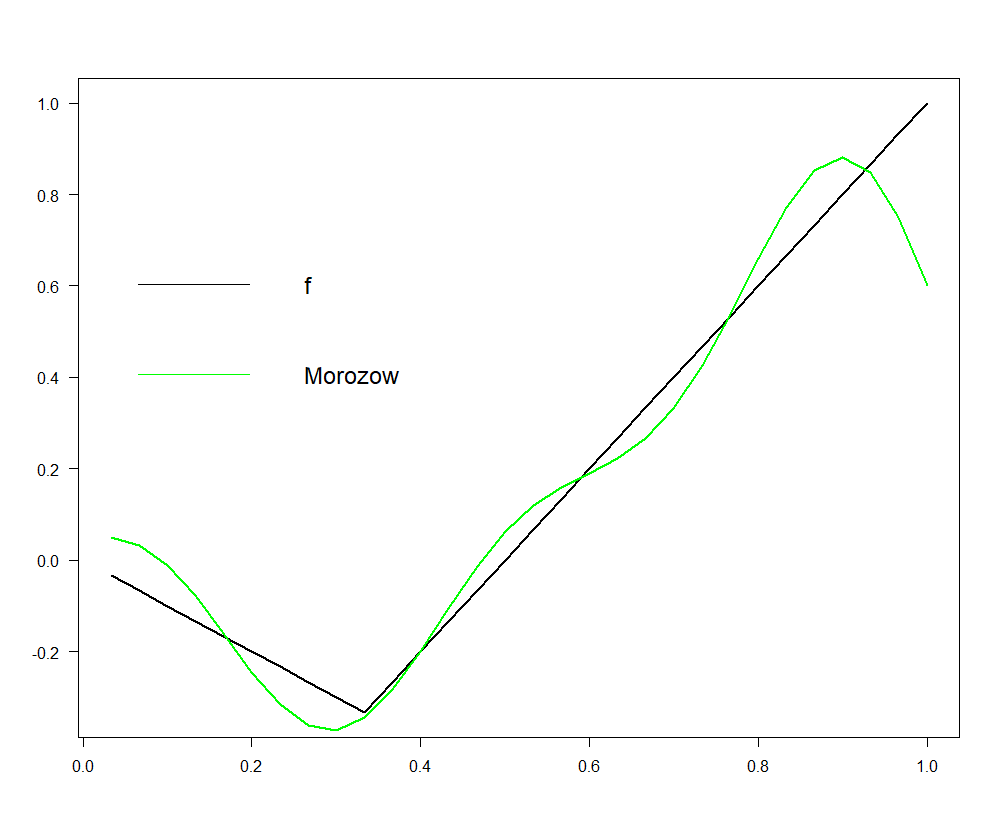
\includegraphics[width=0.4\linewidth]{m}
\captionof{figure}{\color{Green}Zasada rozbieżności Morozowa}
\end{center}
Natomiast w przypadku zastosowania kryterium zaproponowanego przez Cavaliera i in. otrzymano poniższy wynik
\begin{center}
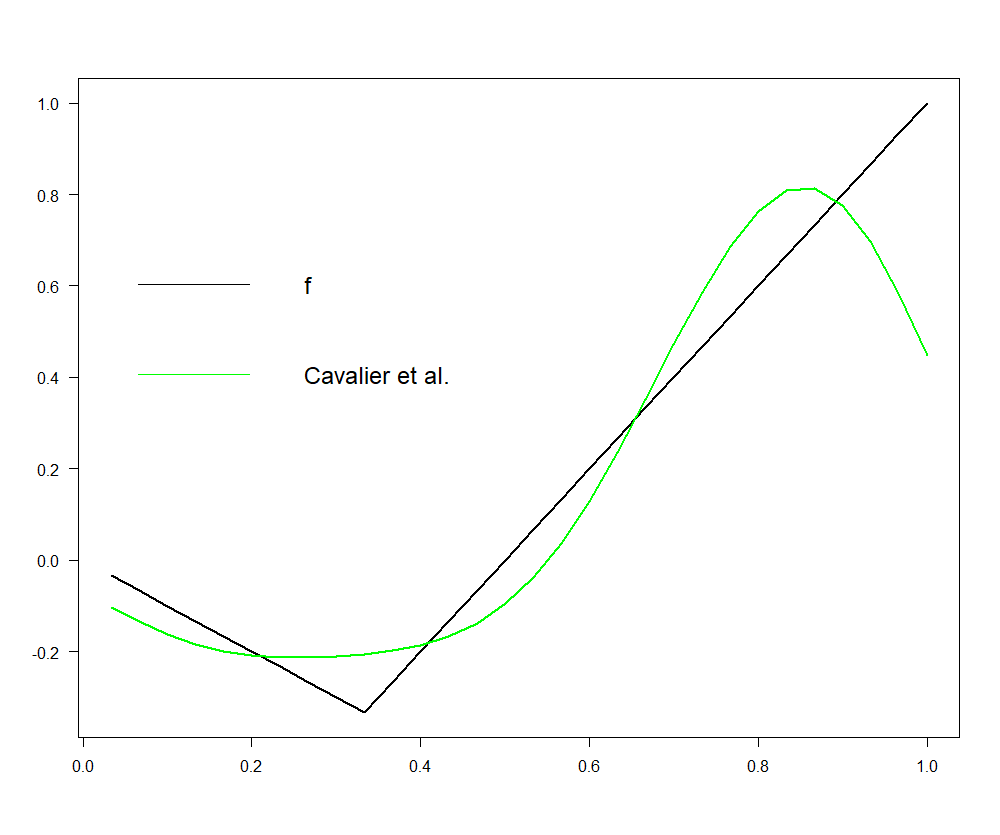
\includegraphics[width=0.4\linewidth]{c}
\captionof{figure}{\color{Green}Cavalier et al.}
\end{center}

\color{SaddleBrown} 

\section*{Wnioski}
W rozważanym eksperymencie metoda zaproponowana przez Cavalier i in. dała nieznacznie gorsze wyniki objawiające się wielkością średniego błędu rozwiązania $\mathbb{E}\norm{f-f_k}\approx 0.58$ w porównaniu do błędu zasady Morozowa na poziomie $0.43$ przy $10\ 000$ powtórzeń eksperymentu. Różnica ta jednak jest nieistotna statystycznie. Na poniższym wykresie zaprezentowano wykresy rozkładu błędów dla obu metod
\begin{center}
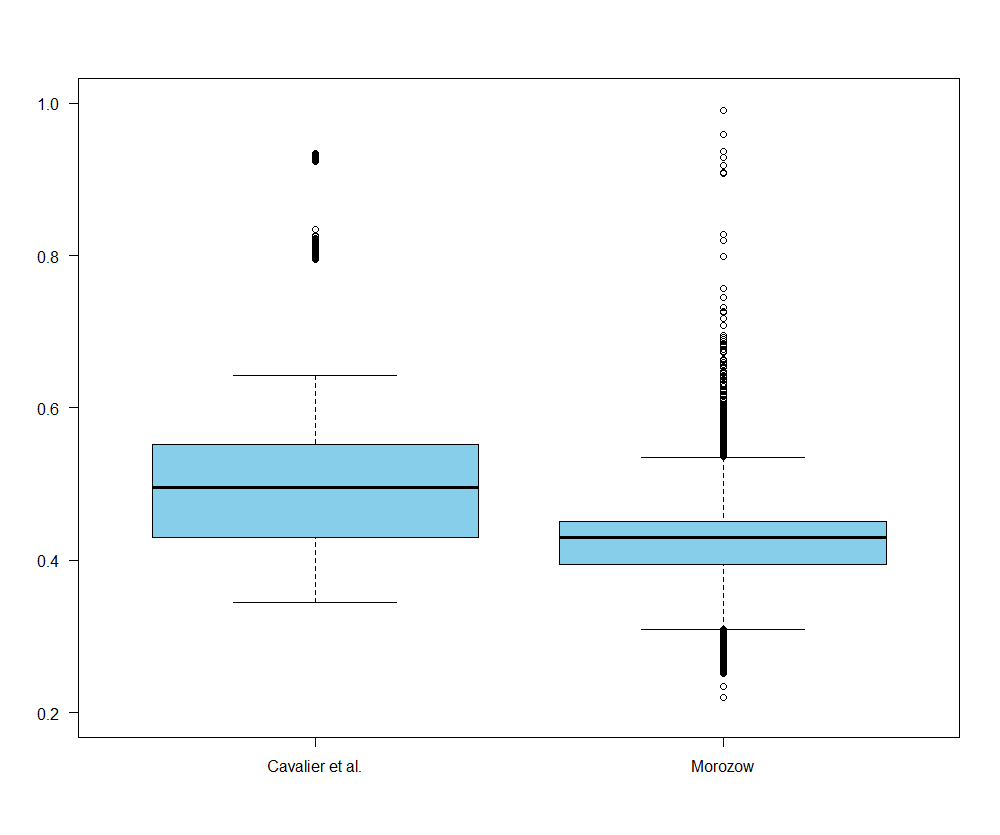
\includegraphics[width=0.4\linewidth]{p}
\captionof{figure}{\color{Green}Podsumowanie wyników}
\end{center}
\color{DarkSlateGray} 


\begin{thebibliography}{5}
\bibitem{iphde} P. Alquier,	E. Gautier, G. Stoltz, \emph{Inverse Problems and High-Dimensional Estimation}	Springer-Verlag, 2011, wydanie zbiorowe,
\bibitem{cavalier1} L. Cavalier, G. K. Golubev, D. Picard, A.B. Tsybakov, \emph{Oracle inequalities for inverse problems}, The Annals of Statistics, Vol. 30, No. 3, 2002, pp. 843–874,	
\bibitem{kaipo}
J. Kaipo, E. Somersalo, \emph{Statistical and computational inverse problems}, Springer, 2004.
\end{thebibliography}

%----------------------------------------------------------------------------------------
%	ACKNOWLEDGEMENTS
%----------------------------------------------------------------------------------------

\section*{Podziękowania}
Chciałbym serdecznie podziękować mojemu Promotorowi Prof. Zbigniewowi Szkutnikowi za pomoc i pokierowanie moim rozwojem naukowym.
%----------------------------------------------------------------------------------------

\end{multicols}
\end{document}